\documentclass[12pt,a4paper]{article}

\usepackage[utf8]{inputenc}
\usepackage[T1]{fontenc}
\usepackage[french]{babel}
\usepackage{textcomp}
\usepackage{amsmath}
\usepackage{amssymb}
\usepackage{graphicx}
\usepackage{float}
\usepackage{geometry}
\usepackage{hyperref}
\usepackage{booktabs}
\usepackage{array}
\usepackage{caption}
\usepackage{subcaption}
\usepackage{listings}
\usepackage{xcolor}
\usepackage{fancyhdr}
\usepackage{titlesec}
\usepackage{parskip}

\geometry{
  top=2.5cm,
  bottom=2.5cm,
  left=2.5cm,
  right=2.5cm,
  headheight=15pt
}

\pagestyle{fancy}
\fancyhf{}
\rhead{Dimensionnement d'un regulateur PI pour un moteur à courant continu}
\lhead{HEPIA}
\graphicspath{ {./ressources/images/} }

\rfoot{\thepage}

\lstset{
  language=Matlab,
  basicstyle=\ttfamily\small,
  keywordstyle=\color{blue},
  commentstyle=\color{green!60!black},
  stringstyle=\color{orange},
  numbers=left,
  numberstyle=\tiny\color{gray},
  breaklines=true,
  frame=single,
  backgroundcolor=\color{gray!10}
}

\hypersetup{
  colorlinks=true,
  linkcolor=blue,
  urlcolor=blue,
  citecolor=blue
}

% --------------------------------------------------------------------------
\begin{document}

% ===== PAGE DE TITRE =====
\begin{titlepage}
  \centering
  \vspace*{2cm}
  {\scshape\Large HEPIA \par}
  \vspace{0.5cm}
  {\large Automatique \& Régulation\par}
  \vspace{2cm}
  \rule{\linewidth}{0.5pt}\\[0.4cm]
  {\huge\bfseries Laboratoire \#4\par}
  \vspace{0.3cm}
  {\Large\bfseries Dimensionnement d'un régulateur\\pour un moteur à courant continu\par}
  \rule{\linewidth}{0.5pt}\\[1.5cm]
  \vfill
  {\large Genève, \today\par}
\end{titlepage}

% ===== TABLE DES MATIÈRES =====
\tableofcontents
\newpage

% --------------------------------------------------------------------------
\section{Introduction}

Les moteurs électriques à courant continu (MCC) sont omniprésents dans l'industrie : robots, véhicules
électriques, systèmes d'entraînement CNC, etc. Ce laboratoire a pour but d'appliquer les méthodes de
dimensionnement de régulateurs vues en cours afin d'imposer une consigne de vitesse à un tel moteur.

\\\\
Les objectifs de ce rapport sont donc d'établir la fonction de transfert du système en boucle ouverte afin de pouvoir dimensionner en un second temps un régulateur (PI) au système.Nous simulons ainsi la boucle fermée sous Simulink et vérifions le dimensionnement effectué de manière théorique. Enfin, nous implémentons le régulateur sur une installation réelle pour établir le lien entre la simulation et la pratique.

% --------------------------------------------------------------------------
\section{Description du système}

Le système est constitué d'un amplificateur (Gélé), d'un moteur à courant continu (Gmot) et d'un capteur de vitesse (Gmes). Les fonctions de transfert des différents blocs sont :

\[
  G_{\text{mot}}(s) = \frac{4{,}53 \cdot 10^{3}}{1 + s \cdot 8 \cdot 10^{-3}}
  \qquad
  G_{\text{élé}}(s) = \frac{20{,}8 \cdot 10^{-3}}{1 + s \cdot 1 \cdot 10^{-3}}
  \qquad
  G_{\text{mes}} = 10{,}7 \cdot 10^{-3}
\]

dont les paramètres sont définis tel que 
\[
    $K_{\text{mot}}$ = $4{,}53 \cdot 10^3$,
    \quad
    $T_1$ = $8 ms, 
    \quad
    $K_{\text{élé}}$ = $20{,}8 \cdot 10^{-3}$,
    \quad
    $T_{\text{élé}}$ = $1 ms,
    \quad
    $K_{\text{mes}}$ = $10{,}7 \cdot 10^{-3}$
\]

% --------------------------------------------------------------------------
\section{A : Fonction de transfert du système (TO CHECK)}

En négligeant le régulateur pour l'instant, la chaîne directe est :

\[
  G_{\text{sys}}(s) = G_{\text{élé}}(s) \cdot G_{\text{mot}}(s)
  = \frac{K_{\text{élé}} \cdot K_{\text{mot}}}{(1 + s T_{\text{élé}})(1 + s T_1)}
\]

Le gain statique de la boucle ouverte sans le régulateur est :

\[
  K_s = K_{\text{mot}} \cdot K_{\text{élé}} \cdot K_{\text{mes}}
  = 4530 \cdot 20{,}8 \cdot 10^{-3} \cdot 10{,}7 \cdot 10^{-3}
  \approx 1{,}008
\]

Alors, la fonction de transfert en boucle ouverte est :

\[
  G_{\text{BO}}(s) = G_R(s) \cdot \frac{K_{\text{élé}} \cdot K_{\text{mot}} \cdot K_{\text{mes}}}
  {(1 + s \cdot 10^{-3})(1 + s \cdot 8 \cdot 10^{-3})}
\]

% --------------------------------------------------------------------------
\section{B : Dimensionnement du régulateur}

Nous souhaitons un dépassement maximal de $D \leq 5\,\%$ sur la réponse indicielle avec un écart statique nul.

\\\\
Cela nous pousse à choisir un régulateur PI, car il permet d'annuler l'écart statique sans perturbation intégrale dans la chaîne directe dont la fonction de transfert est :

\[
  G_R(s) = K_p \left(1 + \frac{1}{T_n s}\right) = \frac{K_p (1 + T_n s)}{T_n s}
\]

Pour compenser le pôle dominant, nous choisissons $T_n = T_1 = 8 \cdot 10^{-3}$\,s. La boucle ouverte compensée devient un système du premier ordre avec intégration :

\[
  G_{\text{BO,comp}}(s) = \frac{K_p \cdot K_s}{T_n \cdot s \cdot (1 + s \cdot 10^{-3})}
  \approx \frac{K_p \cdot K_s}{T_n \cdot s}
  \quad \text{(pour } \omega \ll 1000\,\text{rad/s)}
\]

Un dépassement de 5\,\% correspond à un facteur d'amortissement $\zeta \approx 0{,}69$, soit une marge de phase $\varphi_m \approx 65^{\circ}$.

En appliquant la méthode de Bode avec le modèle de second ordre équivalent, on obtient la constante intégrale :

\[
  T_i = 2 \cdot K_s \cdot T_2
\]

où $T_2 = 1 \cdot 10^{-3}$\,s déterminer directement la constante de temps de l'amplificateur. Nous obtenons alors numériquement pour $T_i$ et $K_p$ :

\[
  T_i = 2 \cdot 1{,}008 \cdot 1 \cdot 10^{-3} \approx 2{,}016 \cdot 10^{-3}\,\text{s}
\]

\[
  K_p = \frac{T_n}{T_i} = \frac{8 \cdot 10^{-3}}{2{,}016 \cdot 10^{-3}} \approx 3{,}97
\]
\newpage
% --------------------------------------------------------------------------
\section{C : Simulation Simulink}

La boucle de régulation a été modélisée sous Simulink avec le régulateur PI calculé précédemment est visible sur Fig. \ref{fig:schema_simulink}.

\begin{figure}[H]
  \centering
  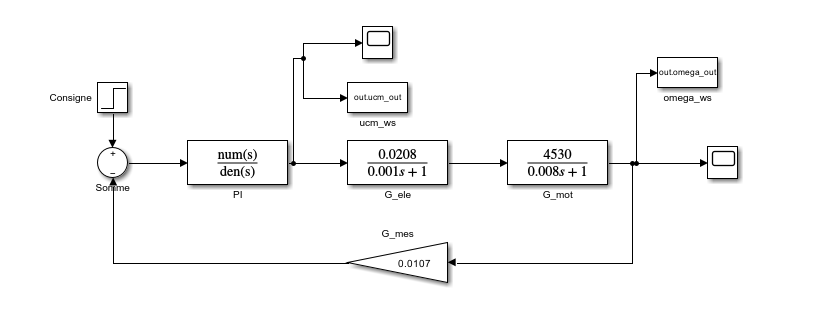
\includegraphics[width=0.85\textwidth]{schema_simulink.png}
  \caption{Schéma Simulink de la boucle de régulation de vitesse}
  \label{fig:schema_simulink}
\end{figure}
Un échelon de consigne de 0 à 10\,rad/s est appliqué. Fig. \ref{fig:step_dep} montre la réponse indicielle théorique obtenue par la simulation Simulink.

\begin{figure}[H]
  \centering
  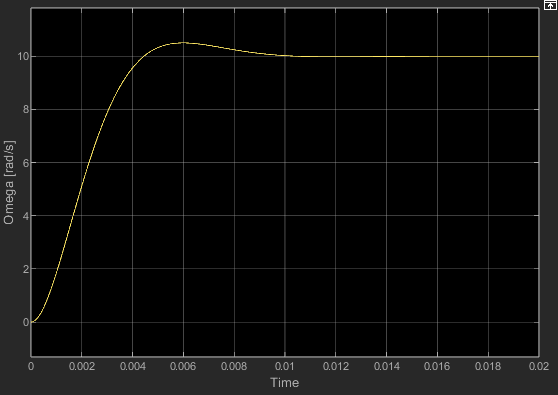
\includegraphics[width=0.75\textwidth]{step_depassement_mot.png}
  \caption{Zoom sur le dépassement de la réponse indicielle simulée}
  \label{fig:step_dep}
\end{figure}

\newpage
Dont nous pouvons visualiser les paramètres depuis Matlab sur Fig. \ref{fig:B_step}.
\begin{figure}[H]
  \centering
    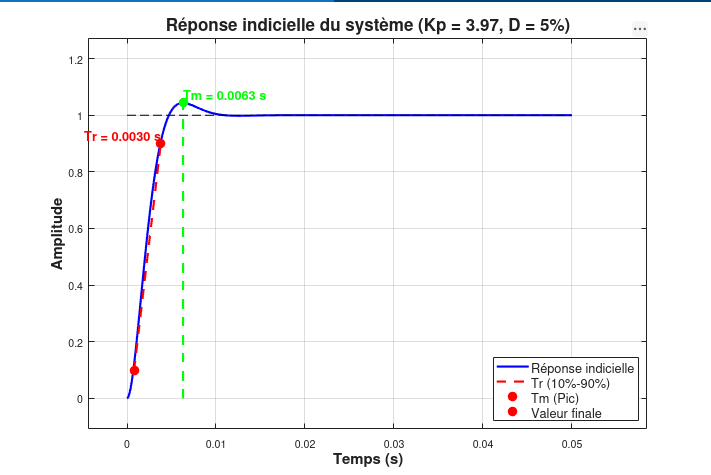
\includegraphics[scale=0.6]{B_step.png}
    \caption{Réponse indicielle simulée}
  \label{fig:B_step}
\end{figure}

Le temps de réponse à 5\,\% vaut environ $T_r \approx 6$\,ms, ce qui est cohérent avec les constantes de temps du système obtenues théoriquement par :
\[
    hello = completer
\]

\newpage
% --------------------------------------------------------------------------
\section{D : Tension de commande $u_{cm}$}

La figure~\ref{fig:step_commande} montre l'évolution de la tension de commande $u_{cm}$ lors de l'application
de l'échelon de consigne (0 à 10\,rad/s).

\begin{figure}[H]
  \centering
  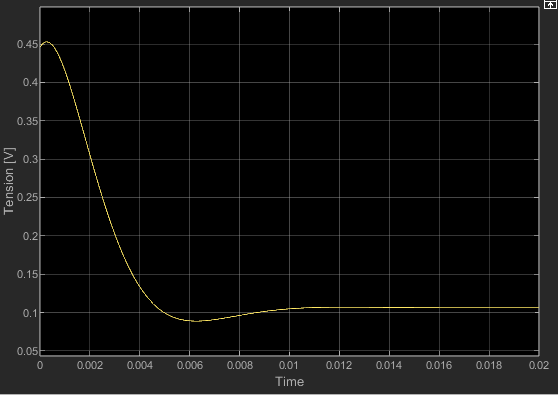
\includegraphics[width=0.75\textwidth]{step_commande.png}
  \caption{Tension de commande $u_{cm}$ lors du saut de consigne 0 $\to$ 10\,rad/s}
  \label{fig:step_commande}
\end{figure}

La tension maximale est $u_{cm,\text{max}} \approx 0{,}46$\,V. Cette valeur est largement dans la plage
acceptable de l'amplificateur (typiquement $\pm 10$\,V), ce qui signifie que le régulateur ne sature
pas lors du démarrage. La commande est donc pleinement linéaire et les performances simulées sont
représentatives du comportement réel attendu.

\newpage
% --------------------------------------------------------------------------
\section{E-F-G-H-I : Implémentation sur l'installation réelle}

Le schéma Simulink \texttt{SIRAu\_PI\_vit.mdl} a été adapté pour intégrer le régulateur PI dimensionné. Les paramètres ont été chargés via le script \texttt{Param\_PI\_Vit.m} compilé run l'expérience sur le PC cible (xPcx quelque chose...).
\\\\
L'expérience sur le PC cible controlant le montage à donc permit de mesurer la réponse en vitesse mesurée sur l'installation réelle. Cela est visible sur Fig. \ref{fig:G_pratique}.

\begin{figure}[H]
  \centering
  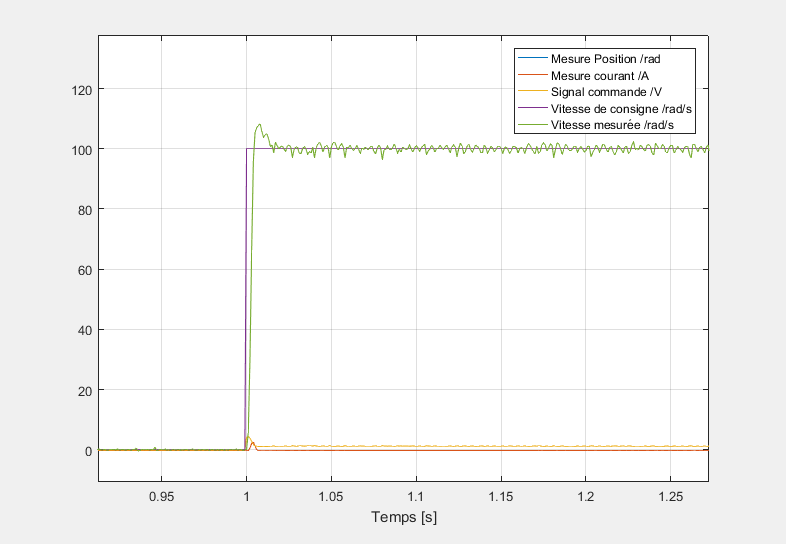
\includegraphics[scale=0.8]{G_fig_pratique.png}
  \caption{Réponse expérimentale -- régulateur PI ($T_2 = 1$\,ms)}
  \label{fig:G_pratique}
\end{figure}


\newpage

Le dépassement observé expérimentalement est d'environ \textbf{7--8\,\%}, contre 5\,\% visé avec le modèle initial. De plus, la qu'avec Simulink (voir Fig. \ref{fig:HI_th2}), nous n'obtenons non-pas $\approx$ 8 \%, mais $\approx$ 15\% de dépassement alors que nous sommes sensés obtenir la même valeur.

\begin{figure}[H]
  \centering
  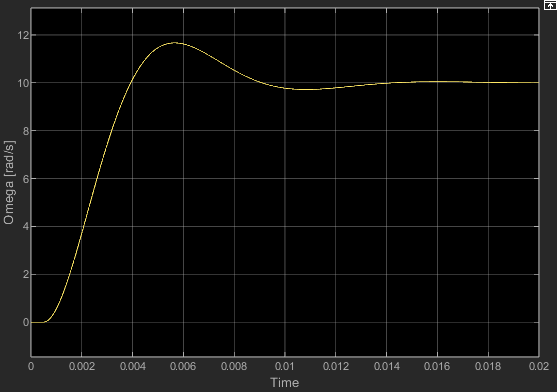
\includegraphics[scale=0.8]{fig_HI_theorique.png}
  \caption{Réponse simulée complète avec retard (vue globale)}
  \label{fig:HI_th2}
\end{figure}

Le gain statique semble être surdimensionné, or les frottements du moteurs sont sensés baisser le gain. Les frottements ralentissent le moteur en basse vitesse mais n'amortissent pas efficacement le dépassement. Ces derniers n'ont pas étés modélisés correctement dans la fonction de transfert du système. Mais comme le montage est vieux, il se peut que le gain du moteur soit plus bas que prévu. Ainsi il vient compenser celui du régulateur et nous obtenons malgré-tout un dépassement relativement juste. L'écart statique est nul et la réponse
converge correctement vers la consigne.
\\\\
Pour palier à ce problème, un retard de $\tau = 0{,}5$\,ms est introduit dans la boucle (voir Fig. \ref{fig:HI_th}).
Ce retard est approximé par une cellule du premier ordre de constante de temps $\tau = 0{,}5$\,ms :

\begin{figure}[H]
  \centering
  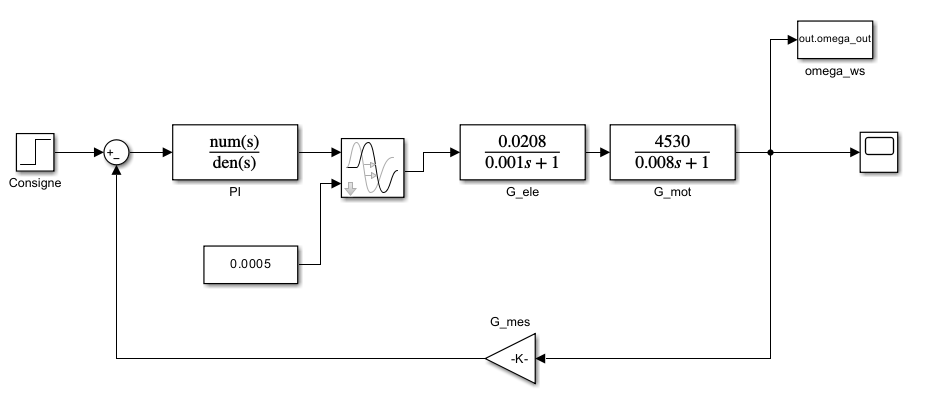
\includegraphics[width=0.75\textwidth]{HI_theorique.png}
  \caption{Réponse indicielle simulée -- régulateur PI avec retard ($T_2 = 1{,}5$\,ms)}
  \label{fig:HI_th}
\end{figure}

\[
  e^{-\tau s} \approx \frac{1}{1 + \tau s} = \frac{1}{1 + 5 \cdot 10^{-4} s}
\]

Ce retard dégrade la marge de phase et nécessite de recalculer le gain $K_p$. On prend désormais
$T_2 = 1{,}5 \cdot 10^{-3}$\,s (somme de la constante de temps de l'amplificateur et du retard) :

\[
  T_i^{\text{new}} = 2 \cdot K_s \cdot T_2 = 2 \cdot 1{,}008 \cdot 1{,}5 \cdot 10^{-3}
  \approx 3{,}024 \cdot 10^{-3}\,\text{s}
\]

\[
  K_p^{\text{new}} = \frac{T_n}{T_i^{\text{new}}} = \frac{8 \cdot 10^{-3}}{3{,}024 \cdot 10^{-3}}
  \approx 2{,}65
\]

Le gain proportionnel est donc réduit par rapport au cas sans retard, ce qui est cohérent : on
sacrifie une partie de la rapidité pour retrouver la marge de phase souhaitée.

Ainsi, nous observons sur Fig. \ref{fig:H_pratique} que le dépassement est ramené à un niveau acceptable ($\leq 5\,\%$) avec le
nouveau jeu de paramètres.


\begin{figure}[H]
  \centering
  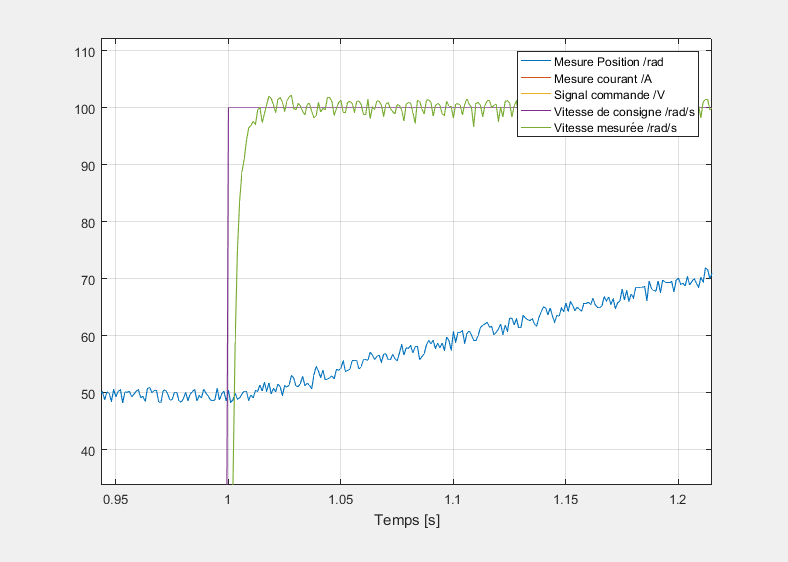
\includegraphics[width=0.75\textwidth]{H_fig_pratique.png}
  \caption{Réponse expérimentale -- régulateur PI avec retard ($T_2 = 1{,}5$\,ms)}
  \label{fig:H_pratique}
\end{figure}

\subsection{Comparaison et analyse}

\begin{table}[H]
  \centering
  \caption{Comparaison des résultats expérimentaux}
  \begin{tabular}{lccc}
    \toprule
    & \textbf{Simulation} & \textbf{Expérience G} & \textbf{Expérience H} \\
    & (sans retard) & ($T_2=1$\,ms) & ($T_2=1{,}5$\,ms) \\
    \midrule
    Dépassement & $\leq 5\,\%$ & $\approx 7$--$8\,\%$ & $\approx 0\,\%$ \\
    Écart statique & 0 & 0 & 0 \\
    Rapidité & $T_r \approx 6$\,ms & bonne & légèrement réduite \\
    $K_p$ & 3,97 & 3,97 & 2,65 \\
    \bottomrule
  \end{tabular}
\end{table}

La prise en compte du retard dans le dimensionnement (tâche H) a permis d'éliminer le dépassement
sur l'installation réelle. En revanche, la réponse est légèrement plus lente, ce qui est le compromis
classique entre rapidité et stabilité (marge de phase).

Les frottements du moteur jouent également un rôle : ils amortissent naturellement les oscillations
et peuvent expliquer pourquoi le dépassement en G était de 7--8\,\% seulement (et non pas plus
élevé), et pourquoi en H on observe une réponse sans dépassement alors que la simulation en prédit un
faible mais non nul.

% --------------------------------------------------------------------------
\section{Conclusion}

Ce laboratoire a permis d'appliquer une démarche complète de dimensionnement d'un régulateur PI
pour un moteur à courant continu :

\begin{enumerate}
  \item La \textbf{fonction de transfert} du système a été établie à partir des modèles linéarisés
    des différents sous-systèmes.
  \item Un \textbf{régulateur PI} a été dimensionné par compensation du pôle dominant (méthode de
    Bode), permettant d'obtenir un dépassement théorique de 5\,\% et un écart statique nul.
  \item La \textbf{simulation Simulink} a validé les performances ($T_r \approx 6$\,ms,
    $u_{cm,\text{max}} \approx 0{,}46$\,V, largement dans les limites de l'amplificateur).
  \item L'\textbf{expérience sur l'installation réelle} a montré un dépassement légèrement supérieur
    (7--8\,\%) dû principalement au retard numérique et aux frottements non modélisés.
  \item La \textbf{prise en compte du retard} dans le redimensionnement a conduit à réduire le gain
    ($K_p : 3{,}97 \to 2{,}65$), ce qui a éliminé le dépassement expérimental au prix d'une légère
    diminution de la rapidité.
\end{enumerate}

Cette expérience illustre bien l'importance de modéliser correctement tous les éléments du système
(y compris les retards de calcul) pour obtenir un comportement en boucle fermée conforme au cahier
des charges.


\end{document}
